%TO DO
%Trägheitsmoment Einheiten?
%Fehler erklären?

\newpage
\section{Auswertung}
Zu Beginn, muss das Gesamtträgheitsmoment $\theta_\text{Ges}$ ermittelt werden.
Dies ergibt sich aus dem Trägheitsmoment der Kugel $\theta_\text{Kugel}$ (aus Gleichung \ref{eqn:trägheitsmoment}) und
dem Trägheitsmoment der Kugelhalterung $\theta_\text{Halterung}$.
\begin{gather*}
    \theta_\text{Kugel}=0.51220 \pm 0.00020\;\mathrm{kgm^2}\\ %0.51220+/-0.00020
    \theta_\text{Halterung}=2.25\cdot 10^{-6} \;\mathrm{kgm^2}\\ %2.25e-06
    \theta_\text{Ges}=0.51220 \pm 0.00020 \;\mathrm{kgm^2} % 0.51220+/-0.00020
\end{gather*}

\subsection{Das Schubmodul $G$ - Messungen ohne B-Feld}
\begin{table}
    \centering
    \label{tab:tabelle_1}
    \begin{tabular}{p{3cm} | p{2cm}}
    \toprule
    & T(s) \\
    \midrule
    &18,696\\
    &18,699\\
    &18,702\\
    &18,763\\
    &18,699\\
    &18,695\\
    &18,591\\
    &18,647\\
    &18,673\\
    &18,665\\
    &18,663\\
    &18,635\\
    \midrule
    Mittelwert $\bar{T}$ (nach Gl. \ref{eqn:mittelwert}):     & 18,667 \\
    Unsicherheit $\sigma$ (nach Gl. \ref{eqn:unsicherheit}):  & 0,029 \\
    \bottomrule
    \end{tabular}
    \caption{Periodendauer T}
\end{table}
\begin{equation}
    \textrm{Mittelwert: } \bar{T}=\frac{1}{n}\sum_{i=1}^{n}T_\text{i}\\\\
    \label{eqn:mittelwert}
\end{equation}\\
\begin{equation}
    \textrm{Unsicherheit: } \bar{\sigma}=\frac{s}{\sqrt{n}}=\frac{\sqrt{\frac{1}{n-1}\sum_{j=1}^n(T_\text{j}-\bar{T})^2}}{\sqrt{n}}
    \label{eqn:unsicherheit}
\end{equation}


\newpage
\subsubsection{Berechnung des Schubmoduls $G$}
Benötigt werden folgende Werte, um das Schubmodul $G$ nach Gleichung \ref{eqn:schubmodul_formel}
zu bestimmen.
Das Elastizitätsmodul $E$ des Materials sei gegeben.
\begin{table}
    \centering
    \label{tab:tabelle_1}
    \begin{tabular}{p{3cm} | p{1.5cm} | p{1.5cm} | p{1.5cm} | p{1.5cm} |p{1.5cm}}
    \toprule
    & L\;/\;cm & d \;/\;mm & $m_\text{k}$\;/\;g & 2$R_\text{k}$\;/\;mm & E\;/\;$10^{11}$Pa\\
    \midrule
    &66,38 & 0,19 & 512,2 &  50,76  & 2.100\\
    &      & 0,19 &       &         &\\    
    &      & 0,2  &       &         &\\
    &      & 0,2  &       &         &\\
    \midrule
    Mittelwert:    &      & 0,0194 &       &        &\\
    Ungenauigkeit: & 0,07 & 0,0004 & 0,205 & 0,0036 & 0.005\\
    \bottomrule
    \end{tabular}
    \caption{Messunggrößen der Apperatur}
    \label{tab:tabelle_2}
\end{table}

Für das Schubmodul $G$ ergibt sich somit:
\begin{equation*}
    G = (7,3 \pm 0,7 )\cdot 10^{10}\;\mathrm{Pa}
\end{equation*}
%G = (7.3\pm 0.7)e+10
Dies enspricht einem prozentualen Fehler von $9,6\%$ (nach Gl. \ref{eqn:relfehler}).

\subsubsection{Berechnung der Querkontraktionszahl}
Mit der Gleichung \ref{eqn:Beziehung} ergibt sich für die Poissonsche Querkontraktionszahl $\mu$
\begin{equation*}
    \mu = 0,45 \pm 0,13 %ist Einheitslos!
    %0.45+/-0.13
\end{equation*}
Dies entspricht einem prozentualen Fehler von $28,9\%$ (nach Gl. \ref{eqn:relfehler}).

\subsubsection{Berechnung des Kompressionsmoduls Q}
Mit der Gleichung \ref{eqn:Beziehung} 
folgt für das Kompressionsmodul $Q$
\begin{equation*}
    Q = (0,7 \pm 1,7) \cdot 10^{12} \;\mathrm{Pa}
    %(0.7+/-1.7)e+12
\end{equation*}
Dies entspricht einem prozentualen Fehler von $242,8\%$ (nach Gl. \ref{eqn:relfehler}).\\

Der relative Gauß-Fehler ergibt sich dabei aus:
\begin{equation}
    \frac{\Delta x_i}{x_i}=\sqrt{(\frac{\sigma_{k1}}{k_1})^2+(\frac{\sigma_{k2}}{k_2})^2+...} \cdot 100\%
    \label{eqn:relfehler}
\end{equation}

\newpage
\subsection{Das Magnetische Moment - Messung mit B-Feld}

Für das Magnetische Feld $B$ im Inneren einer Helmholtz-Spulen gilt:
\begin{equation}
    B= \frac{8}{\sqrt{125}} \cdot \frac{\mu_0 I N}{R}
\end{equation}
wobei $N=390$ die Windungszahl und $R=78$mm der Radius der Spulen ist.\\
Aus Gleichung \ref{eqn:periode}
folgt:
\begin{equation}
    \to m_\text{mag}B+D := \zeta = \frac{4\pi^2\theta_\text{Ges}}{T^2_\text{m}}
\end{equation}

Damit ist $\zeta$ eine lineare Funktion. Daraus folgen dann die Parameter $m_\text{mag}$, $D$ und $B$.\newline
$\zeta = m_\text{mag}B + D$ \to $f(x)=ax+b$ mit $b = D$ und $a=m_\text{mag}$

Die Messwerte sind auf der folgenden Seite in den Tabellen \ref{tab:tabelle_01A} und \ref{tab:tabelle_06A}
zu finden.
\begin{figure}[h]
    \centering
    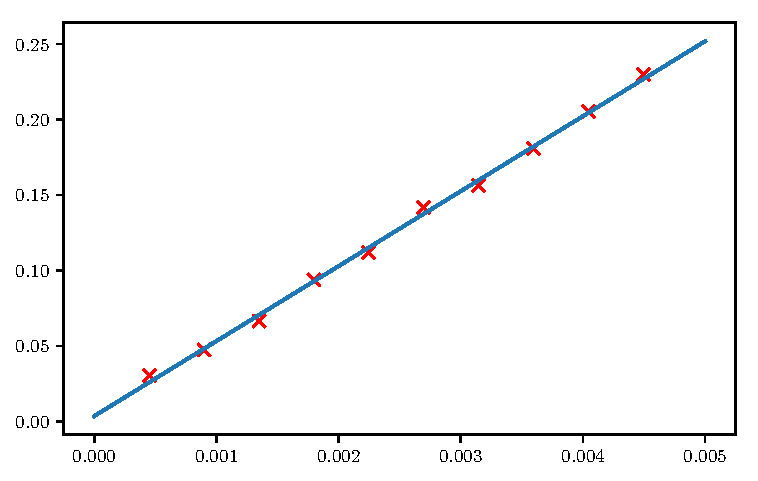
\includegraphics[width=0.85\textwidth, height=0.5\textwidth]{build/plot.pdf}
    \caption{$\zeta$-B-Diagramm}        
    \label{fig:Diagramm}
\end{figure}

Somit ergibt sich:
\begin{gather*}
    m_\text{mag} = 0,05 \pm 8,41 \cdot 10^{-4} \;\mathrm{\frac{kgm^2}{Ts^2}}\\\\
    D = 3,55\cdot10^{-6} \pm 2,35 \cdot 10^{-6} \;\mathrm{\frac{kgm^2}{s^2}}
\end{gather*}

\newpage
\begin{table}
    \caption{Periodendauer T des Drahtes mit B-Feld von 0,1A - 0,5A}
    \centering
    \begin{tabular}{p{3cm} | p{1.5cm} p{1.5cm} p{1.5cm} p{1.5cm} p{1.5cm}}
    I & 0,1A & 0,2A & 0,3A & 0,4A & 0,5A\\
    \midrule
    T\;/\;s & 13,168 & 10,583 & 8,871 &  7,444 &  6,639\\   
    & 13,156 & 10,577 & 8,873 &  7,444 &  6,856\\   
    & 13,151 & 10,564 & 8,869 &  7,465 &  6,840\\   
    & 13,140 & 10,565 & 8,864 &  7,436 &  6,849\\   
    & 13,130 & 10,558 & 8,860 &  7,440 &  6,860\\   
    & 13,103 & 10,552 & 8,855 &  7,462 &  6,855\\   
    & 13,069 & 10,530 & 8,850 &  7,440 &  6,850\\   
    & 13,085 & 10,527 & 8,842 &  7,463 &  6,842\\   
    & 13,074 & 10,518 & 8,835 &  7,445 &  6,835\\   
    & 13,011 &  9,773 & 8,823 &  7,428 &  6,823\\ 
    \midrule
    Mittelwert $\bar{T}\;/\;s$ (nach Gl. \ref{eqn:mittelwert}):    & 13,109 & 10,475 & 8,854 & 7,447 & 6,825 \\
    \midrule
    B-Feld \;/\;T: & 4,50E-04 & 8,99E-04 & 1,35E-03 & 1,80E-03 & 2,25E-03\\
    $\zeta\;/\;\frac{kgm^2}{s^2}$: & 3,08E-05 & 4,83E-05 & 6,76E-05 & 9,56E-05 & 1,14E-04\\
    \bottomrule
    \end{tabular}
    \label{tab:tabelle_01A}
\end{table}



\begin{table}[h!]
    \centering
    \caption{Periodendauer T des Drahtes mit B-Feld von 0,6A - 1,0A}
    \begin{tabular}{p{3cm} | p{1.5cm} p{1.5cm} p{1.5cm} p{1.5cm} p{1.5cm}}
    I & 0,6A & 0,7A & 0,8A & 0,9A & 1,0A\\
    \midrule
    T\;/\;s  & 4,722 &  5,777 &  5,384 &  5,018 &  4,733\\
    & 6,237 &  5,767 &  5,378 &  5,029 &  4,779\\
    & 6,261 &  5,784 &  5,376 &  5,077 &  4,747\\
    & 6,227 &  5,767 &  5,362 &  5,045 &  4,765\\
    & 6,208 &  5,795 &  5,376 &  5,008 &  4,762\\
    & 6,229 &  5,762 &  5,363 &  5,038 &  4,728\\
    & 6,227 &  5,774 &  5,368 &  5,052 &  4,777\\
    & 6,178 &  5,784 &  5,359 &  5,061 &  4,756\\
    & 6,183 &  5,761 &  5,364 &  5,034 &  4,792\\
    & 6,163 &  5,791 &  5,373 &  5,028 &  4,789\\
    \midrule
    Mittelwert $\bar{T}\;/\;s$ (nach Gl. \ref{eqn:mittelwert}):    & 6,064 & 5,776 & 5,370 & 5,039 &  4,763 \\
    \midrule
    B-Feld \;/\;T: & 2,70E-03 & 3,15E-03 & 3,60E-03 & 4,05E-03 & 4,50E-03 \\      
    $\zeta\;/\;\frac{kgm^2}{s^2}$: & 1,44E-04 & 1,59E-04 & 1,84E-04 & 2,09E-04 & 2,34E-04\\
    \bottomrule
    \end{tabular}
    \label{tab:tabelle_06A}
\end{table}

\label{sec:Auswertung}
